%-----------------------------------LICENSE------------------------------------%
%   This file is part of Mathematics-and-Physics.                              %
%                                                                              %
%   Mathematics-and-Physics is free software: you can redistribute it and/or   %
%   modify it under the terms of the GNU General Public License as             %
%   published by the Free Software Foundation, either version 3 of the         %
%   License, or (at your option) any later version.                            %
%                                                                              %
%   Mathematics-and-Physics is distributed in the hope that it will be useful, %
%   but WITHOUT ANY WARRANTY; without even the implied warranty of             %
%   MERCHANTABILITY or FITNESS FOR A PARTICULAR PURPOSE.  See the              %
%   GNU General Public License for more details.                               %
%                                                                              %
%   You should have received a copy of the GNU General Public License along    %
%   with Mathematics-and-Physics.  If not, see <https://www.gnu.org/licenses/>.%
%------------------------------------------------------------------------------%
%   Author:     Ryan Maguire                                                   %
%   Date:       December 6, 2024                                               %
%------------------------------------------------------------------------------%
\documentclass{beamer}
\usepackage{amsmath}
\graphicspath{{../images/}}
\title{Tait Graphs for Virtual Knots}
\author{Ryan Maguire}
\date{December 8, 2024}
\usenavigationsymbolstemplate{}
\setbeamertemplate{footline}[frame number]
\graphicspath{{../images/}}
\begin{document}
    \maketitle
    \begin{frame}{Outline}
        \begin{itemize}
            \item Tait Graphs for Classical Knots.
            \item What are Virtual Knots?
            \item Tait Graphs for Virtual Knots.
            \item The Jones Polynomial via Tait Graphs.
        \end{itemize}
        This talk is mostly pictures, I hope you enjoy.
    \end{frame}
    \begin{frame}{Tait Graphs for Classical Knots}
        We start with a link diagram (oriented or unoriented), like
        Fig.~\ref{fig:hopf_link_diagram}.
        \begin{figure}
            \centering
            \includegraphics{hopf_link_diagram}
            \label{fig:hopf_link_diagram}
            \caption{An Unoriented Hopf Link}
        \end{figure}
    \end{frame}
    \begin{frame}{Tait Graphs for Classical Knots}
        Pick a random face and place a dot in the middle. For each face that
        is connected to your initial one by going \textit{across} (no going
        left, and no going right) a crossing, place a dot in middle of it as
        well. Keep doing this recursively until there are no new faces to
        put dots in.
        \begin{figure}
            \centering
            \includegraphics{hopf_link_unoriented_tait_graph_001}
            \label{fig:hopf_link_unoriented_tait_graph_001}
            \caption{A Hopf Link with Dots in the Faces}
        \end{figure}
    \end{frame}
    \begin{frame}{Tait Graphs for Classical Knots}
        Every face that has a dot in it, shade the entire region gray, and
        connect any two adjacent dots with an edge, and associate a sign to this
        edge based on the drawings below.
        \begin{figure}
            \centering
            \includegraphics{tait_graph_sign}
            \label{fig:tait_graph_sign}
            \caption{Signing the Edges of the Tait Graph}
        \end{figure}
    \end{frame}
    \begin{frame}{Tait Graphs for Classical Knots}
        To make things more visual, color the negative edges red, and the
        positive edges blue.
        \begin{figure}
            \centering
            \includegraphics{hopf_link_unoriented_tait_graph_002}
            \label{fig:hopf_link_unoriented_tait_graph_002}
            \caption{Tait Graph for the Hopf Link}
        \end{figure}
    \end{frame}
    \begin{frame}{Tait Graphs for Classical Knots}
        Remove the link diagram, and viola, you have a Tait graph.
        \begin{figure}
            \centering
            \includegraphics{hopf_link_tait_graph_no_link_diagram_001}
            \label{fig:hopf_link_tait_graph_no_link_diagram_001}
            \caption{Tait Graph for the Hopf Link}
        \end{figure}
    \end{frame}
    \begin{frame}{Tait Graphs for Classical Knots}
        Depending on your choice of initial face, you may get a different
        graph. There are two possibilities, and they are planar duals.
        \begin{figure}
            \centering
            \resizebox{!}{0.6\textheight}{%
                \includegraphics{%
                    trefoil_tait_graph_with_both_graphs_and_knot_diagram_001
                }
            }
            \label{fig:trefoil_tait_graph_with_both_graphs_and_knot_diagram_001}
            \caption{Tait Graphs for the Right-Handed Trefoil}
        \end{figure}
    \end{frame}
    \begin{frame}{Tait Graphs for Classical Knots}
        This operation reverses, you can go from connected planar graphs to
        knots (Goeritz / Medial construction). The key ingredient is the fact
        that the faces in such a graph are topological disks.
    \end{frame}
    \begin{frame}{Tait Graphs for Classical Knots}
        The Reidemeister moves have simple descriptions in terms of operations
        on Tait graphs. Reidemeister I means you can remove loops and leaves.
        \begin{figure}
            \centering
            \resizebox{!}{0.65\textheight}{%
                \includegraphics{tait_graph_reidemeister_1_dual}
            }
            \caption{R I for Tait Graphs}
        \end{figure}
    \end{frame}
    \begin{frame}{Tait Graphs for Classical Knots}
        \begin{figure}
            \centering
            \includegraphics{tait_graph_reidemeister_1}
            \caption{R I for Tait Graphs}
        \end{figure}
    \end{frame}
    \begin{frame}{Tait Graphs for Classical Knots}
        R II is conservation of charge.
        \begin{figure}
            \centering
            \includegraphics{tait_graph_reidemeister_2_001}
            \caption{R II for Tait Graphs}
        \end{figure}
    \end{frame}
    \begin{frame}{Tait Graphs for Classical Knots}
        R III also comes from electromagnetism, it is the $Y-\Delta$ move.
        \begin{figure}
            \centering
            \includegraphics{tait_graph_reidemeister_3_001}
            \caption{R III for Tait Graphs}
        \end{figure}
    \end{frame}
    \begin{frame}{Tait Graphs for Classical Knots}
        A classic fact is that knot diagrams always yield checkerboard
        patterns on the plane (or sphere). The Tait graph always exists for
        classical knot, and for connected link diagrams.
    \end{frame}
    \begin{frame}{Tait Graphs for Classical Knots}
        Historical uses:
        \begin{enumerate}
            \item Knot enumeration / tabulation (Tait).
            \item Proving the Tait conjecture (Thistlethwaite).
            \item Computing the Jones polynomial (related to 2).
        \end{enumerate}
        \begin{figure}
                \centering
                \resizebox{!}{0.6\textheight}{%
                    \includegraphics{tait_graph_kauffman_negative_smoothing}
                }
                \caption{Kauffman Bracket for Tait Graphs}
        \end{figure}
    \end{frame}
    \begin{frame}{Tait Graphs for Classical Knots}
        Sample calculation.
        \begin{figure}
            \centering
            \includegraphics{twist_knot_tait_graph_kauffman_relation}
            \caption{Jones Polynomial for Twist Knots}
        \end{figure}
    \end{frame}
    \begin{frame}{Tait Graphs for Classical Knots}
        \begin{align}
            \langle{K_{N+1}}\rangle
            &=\langle{K_{N}}\rangle
            -q(-q^{2})^{N}\langle{H}\rangle\\
            &=\langle{K_{N}}\rangle
            +(-1)^{N+1}q^{2N+1}\langle{H}\rangle
        \end{align}
        We may expand this recusion out $N$ times until we get $K_{1}$,
        which is the left-handed trefoil. Our formula becomes:
        \begin{equation}
            \langle{K_{N+1}}\rangle
            =\langle{K_{1}}\rangle
            +\langle{H}\rangle
            \sum_{k=1}^{k}(-1)^{k+1}q^{2k+1}
        \end{equation}
        Using the geometric series we get:
        \begin{equation}
            \langle{K_{N+1}}\rangle
            =\langle{K_{1}}\rangle+\langle{H}\rangle
            \frac{q^{3}}{1+q^{2}}\big(1+(-1)^{N+1}q^{2N}\big)
        \end{equation}
        Where $K_{1}$ is the left-handed trefoil, and $H$ is the Hopf link.
    \end{frame}
    \begin{frame}{Virtual Knots}
        Virtual knots are embeddings of $\mathbb{S}^{1}$ into thickened
        surfaces. They can also be viewed as arbitrary (signed) Gauss codes.
        \par\hfill\par
        For technical reasons, we require $\mathbb{S}^{1}$ is embedded in
        a surface of \textbf{minimal genus}. Classical knots are precisely
        the virtual knots that embed into a thickened sphere.
    \end{frame}
    \begin{frame}{Virtual Knots}
        \begin{figure}
            \centering
            \includegraphics[angle=90]{chain_link_fence_knot_virtual}
            \caption{Chain Link Fence Knot (Virtual)}
        \end{figure}
    \end{frame}
    \begin{frame}{Virtual Knots}
        \begin{figure}
            \centering
            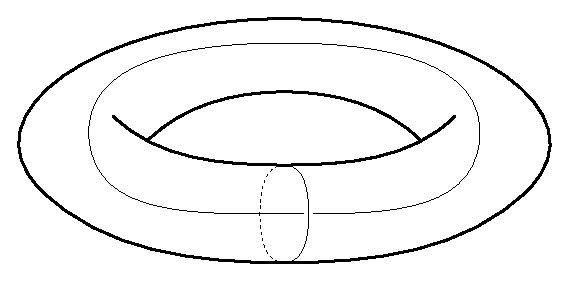
\includegraphics{chain_link_fence_knot_on_torus}
            \caption{Chain Link Fence Knot (Torus)}
        \end{figure}
    \end{frame}
    \begin{frame}{Virtual Knots}
        \begin{figure}
            \centering
            \includegraphics{chain_link_fence_knot_on_flat_torus}
            \caption{Chain Link Fence Knot (Torus)}
        \end{figure}
    \end{frame}
    \begin{frame}{Virtual Knots}
        Why it is called a chain link fence.
        \begin{figure}
            \centering
            \resizebox{!}{0.75\textheight}{%
                \includegraphics{chain_link_fence_knot_on_flat_torus_universal_cover}
            }
            \caption{Chain Link Fence Knot (Universal Cover)}
        \end{figure}
    \end{frame}
    \begin{frame}{Virtual Knots}
        Let's try a first attempt at a Tait graph.
        \begin{figure}
            \centering
            \includegraphics{chain_link_fence_knot_on_flat_torus_tait_graph_naive}
            \caption{Na\"{i}ve Tait Graph for the Chain Link Fence}
        \end{figure}
    \end{frame}
    \begin{frame}{Virtual Knots}
        Uh oh, this spells trouble.
        \begin{figure}
            \centering
            \includegraphics{chain_link_fence_knot_naive_tait_graph}
            \caption{Removing the Torus Structure}
        \end{figure}
    \end{frame}
    \begin{frame}{Virtual Knots}
        Two problems.
        \begin{enumerate}
            \item
                We can no longer apply Reidemeister I moves. Loops have meaning.
            \item
                We lost uniqueness. This is the Tait graph of a Hopf link with
                two loops (R I) moves introcued.
        \end{enumerate}
    \end{frame}
    \begin{frame}{Virtual Knots}
        Solution: Introduce a new type of vertex. A \textit{hollow} vertex
        at each crossing. Solid vertices are then connected to the hollow ones,
        and vice versa. The result is a bipartite multigraph with signed
        edges.
        \begin{figure}
            \centering
            \includegraphics{chain_link_fence_tait_graph}
            \caption{Virtual Tait Graph for the Chain Link Fence Knot}
        \end{figure}
    \end{frame}
    \begin{frame}{Virtual Tait Graphs}
        Properties.
        \begin{enumerate}
            \item Saves R I.
            \item We can copy the medial construction and reverse the process.
        \end{enumerate}
    \end{frame}
    \begin{frame}{Virtual Tait Graphs}
        \begin{theorem}
            If $K$ is a classical knot (virtual genus 0), all hollow vertices
            have degree two.
        \end{theorem}
        \begin{proof}
            The checkerboard pattern makes degree 4 impossible.
        \end{proof}
        Does the converse hold?
    \end{frame}
    \begin{frame}{Virtual Tait Graphs}
        Nope.
        \begin{figure}
            \centering
            \includegraphics{complete_graph_k5_minor_on_flat_torus_001}
            \caption{$K_{5}$ with new hollow vertices}
        \end{figure}
    \end{frame}
    \begin{frame}{Virtual Tait Graphs}
        \begin{figure}
            \centering
            \includegraphics{complete_graph_k5_minor_tait_graph_on_flat_torus_001}
            \caption{The Underlying Virtual Knot}
        \end{figure}
    \end{frame}
    \begin{frame}{Virtual Tait Graphs}
        You can generalize this.
        Take any connected graph, add a hollow vertex to each edge, put the
        graph on a minimal genus surface, and repeat this construction.
    \end{frame}
    \begin{frame}{Virtual Tait Graphs}
        You can also get the Jones polynomial!
    \end{frame}
    \begin{frame}{The End}
        \begin{center}
            Thank you!
        \end{center}
    \end{frame}
\end{document}
